\documentclass[10pt]{book}
\usepackage{graphicx} % Required for inserting images
\usepackage[spanish]{babel}
\usepackage{soul} %Paquete para subrayar texto
\usepackage{amssymb} %Paquete para letras sin relleno y fraktur
\usepackage{mathrsfs} %Paquete para letras cursivas cursivas

\usepackage{amsthm}
\usepackage{amsmath} %Para ecuaciones matematicas
\usepackage{mathtools} %Extiende al paquete amsmath
\usepackage{enumitem}
\usepackage{tikz}
\usepackage{tikz-cd} %Para diagramas conmutativos
\usepackage{hyperref}

%Para corregir el error en la conversion de HTML para Tex4ht
\usepackage{etoolbox}
\AtBeginEnvironment{tikzpicture}{\shorthandoff{>}}
%Eso es en caso de flechas


\theoremstyle{definition}

\newtheorem{defi}{Definición}

\theoremstyle{theorem}
\newtheorem{teo}[defi]{Teorema}

\theoremstyle{remark}

\newtheorem{nota}{Nota}

\title{Pininos en \LaTeX}
\author{Los tres}
\date{\today}



\usepackage[sorting=nyt, style=alphabetic, doi=false,firstinits=true, isbn=false]{biblatex}

\addbibresource{biblio.bib}



\begin{document}

\maketitle

\chapter{Tipografía}

Aquí vamos a mostrar los distintos tamaños de fuentes y sus estilos.
\section{Tamaños de fuentes}

\normalsize Este es el tamaño principal.

{\large El inmediato superior.}

{\Large El inmediato superior.}

{\LARGE El inmediato superior.}

{\huge El más grande.}

{\Huge El más grande.}

Regresamos a tamaño principal.

{\small El inmediato inferior}

{\footnotesize El que sigue para abajo}

{\scriptsize Más chiquito}

{\tiny Chiiquitito}

\section{Estilos}

{\bfseries En negritas} ya no

{\itshape Itálicas} ya no

{\slshape Inclinadas} ya no

{\scshape Versalitas} ya no. Ej. El siglo XXI se acostumbra indacarlo en versalitas, como siglo \textsc{xxi}


{\bfseries\itshape\tiny Chiquitita itálica y negritas }

{\uppercase {Letras en mayúsculas}} %Letras en mayúsculas normales

{\mdseries Texto en grosor intermedio} %Grosor intermedio de letra

Para enfatizar \emph{solo una} palabra en el texto %Enfatiza la palabra cambiando a cursiva si es normal y a normal si el texto esta en cursiva

Así se pueden \ul{subrayar} las cosas. % Texto subrayado (se necesita un paquete)


\section{Familias}\label{sec:familias}

La \textsf{sin patines} (sans-serif) es la family
{\sffamily Texto sin patines}

{\ttfamily Esta es fuente mono espaciada mix} mix

\texttt{prosell@im.unam.mx}

\texttt{gerardoalmazanparra@ciencias.unam.mx}


\subsection{Familias de letras para matemáticas}

Se usan paquetes especiales para usarlas final f{i}\\
Se usan paquetes especiales para usarlas final f{i}

\medskip

Se usan paquetes especiales para usarlas final f{i}
Se usan paquetes especiales para usarlas final f{i}


%\\ al final del parrafo para hacer salto de parrafo

$\mathcal{ABCDEFGH abcdfgh}$ %Letras caligraficpara matematica

$\mathbb{ABCDFGH}$ %Letras sin relleno solo mayusculas

$\mathfrak{abcdfg ABCDFG}$ %Letras "Fraktur"

$\mathscr{ABCDF}$ %Estas se llaman letras formales Ralph Smith segun el manual

Por ejemplo, podemos considerar $\mathcal{F}$ una familia de funciones

\section{Enunciados distinguidos}

\begin{teo}
    Este es mi primer teorema.
\end{teo}
\begin{proof}
    La demostración del teorema $x^2=-1$. Otra forma de poner matemáticas en modo línea es \(x^2-y\) En texto se ve mal: $\frac{-b\pm\sqrt{b^2-4ac}}{2a}$
    \begin{equation*}
        x^2=-1
        %\qedhere
    \end{equation*}
\end{proof}

\begin{defi}
    Una definición es una definición.
\end{defi}
\[
x=\frac{-b\pm\sqrt{b^2-4ac}}{2a}
\]
\begin{nota}
    Esta es una observación.
\end{nota}
$$
x=\frac{-b\pm\sqrt{b^2-4ac}}{2a}
$$
\begin{defi}
    Otra definición
\end{defi}

\section{Listas}

\begin{itemize}
    \item Un elemento
    \item Otro
    \item Y otro más
\end{itemize}

\begin{proof}
\leavevmode
\begin{enumerate}
    \item Primer elemento
    \item Segundo elemento
    \item Tercero
\qedhere
\end{enumerate}
\end{proof}

\medskip
{\bfseries Otras listas}
% \renewcommand{\theenumi}{\Roman{enumi}}
% \renewcommand{\theenumii}{\roman{enumii}} %Preguta
% \renewcommand{\labelenumiii}{$\bigstar$}

\begin{enumerate}[label={(\Alph*)},itemsep=0pt]
    \item Un elemento
    \begin{enumerate}
        \item Segundo elemento
        \begin{itemize}[label={$\bigstar$}]
            \item otro
            \item otro diferente
        \end{itemize}
        \item Tercer elemento. Como aparece en texto , texto y ás texto más G.~Almazán \ref{sec:familias}

        \cite{lamport,nuestro}.

    \end{enumerate}
    \item Otro
    \begin{enumerate}
        \item Segundo elemento
        \item Tercer elemento
    \end{enumerate}
    \item Y otro más
\end{enumerate}

\chapter{Paquetes chidos}

\begin{description}[font=\sffamily]
    \item[enumitem] Modificar listas. Se usa parámetros opcionales después de \verb+\begin{lista}[parámetros]+. Podemos modificar el símbolo de enumeración, espacios entre elementos y márgenes, etc.
    \item[biblatex] Bibliografía usando base de datos.\cite{lamport}
     \item[hyperref] Hipervínculos internos y externos en el documento
    \item[graphicx] Permite insertar y manipular imágenes.
    \item[tikZ] Para gráficos
    \item[tikzcd] Para dibujar diagramas conmutativos.

\end{description}


\section{Ejemplos de los paquetes}

\subsection{Insertar imágenes}
Se insertan imágenes con el paquete {\bfseries {\sffamily graphicx}}.

\begin{figure}
    \centering
    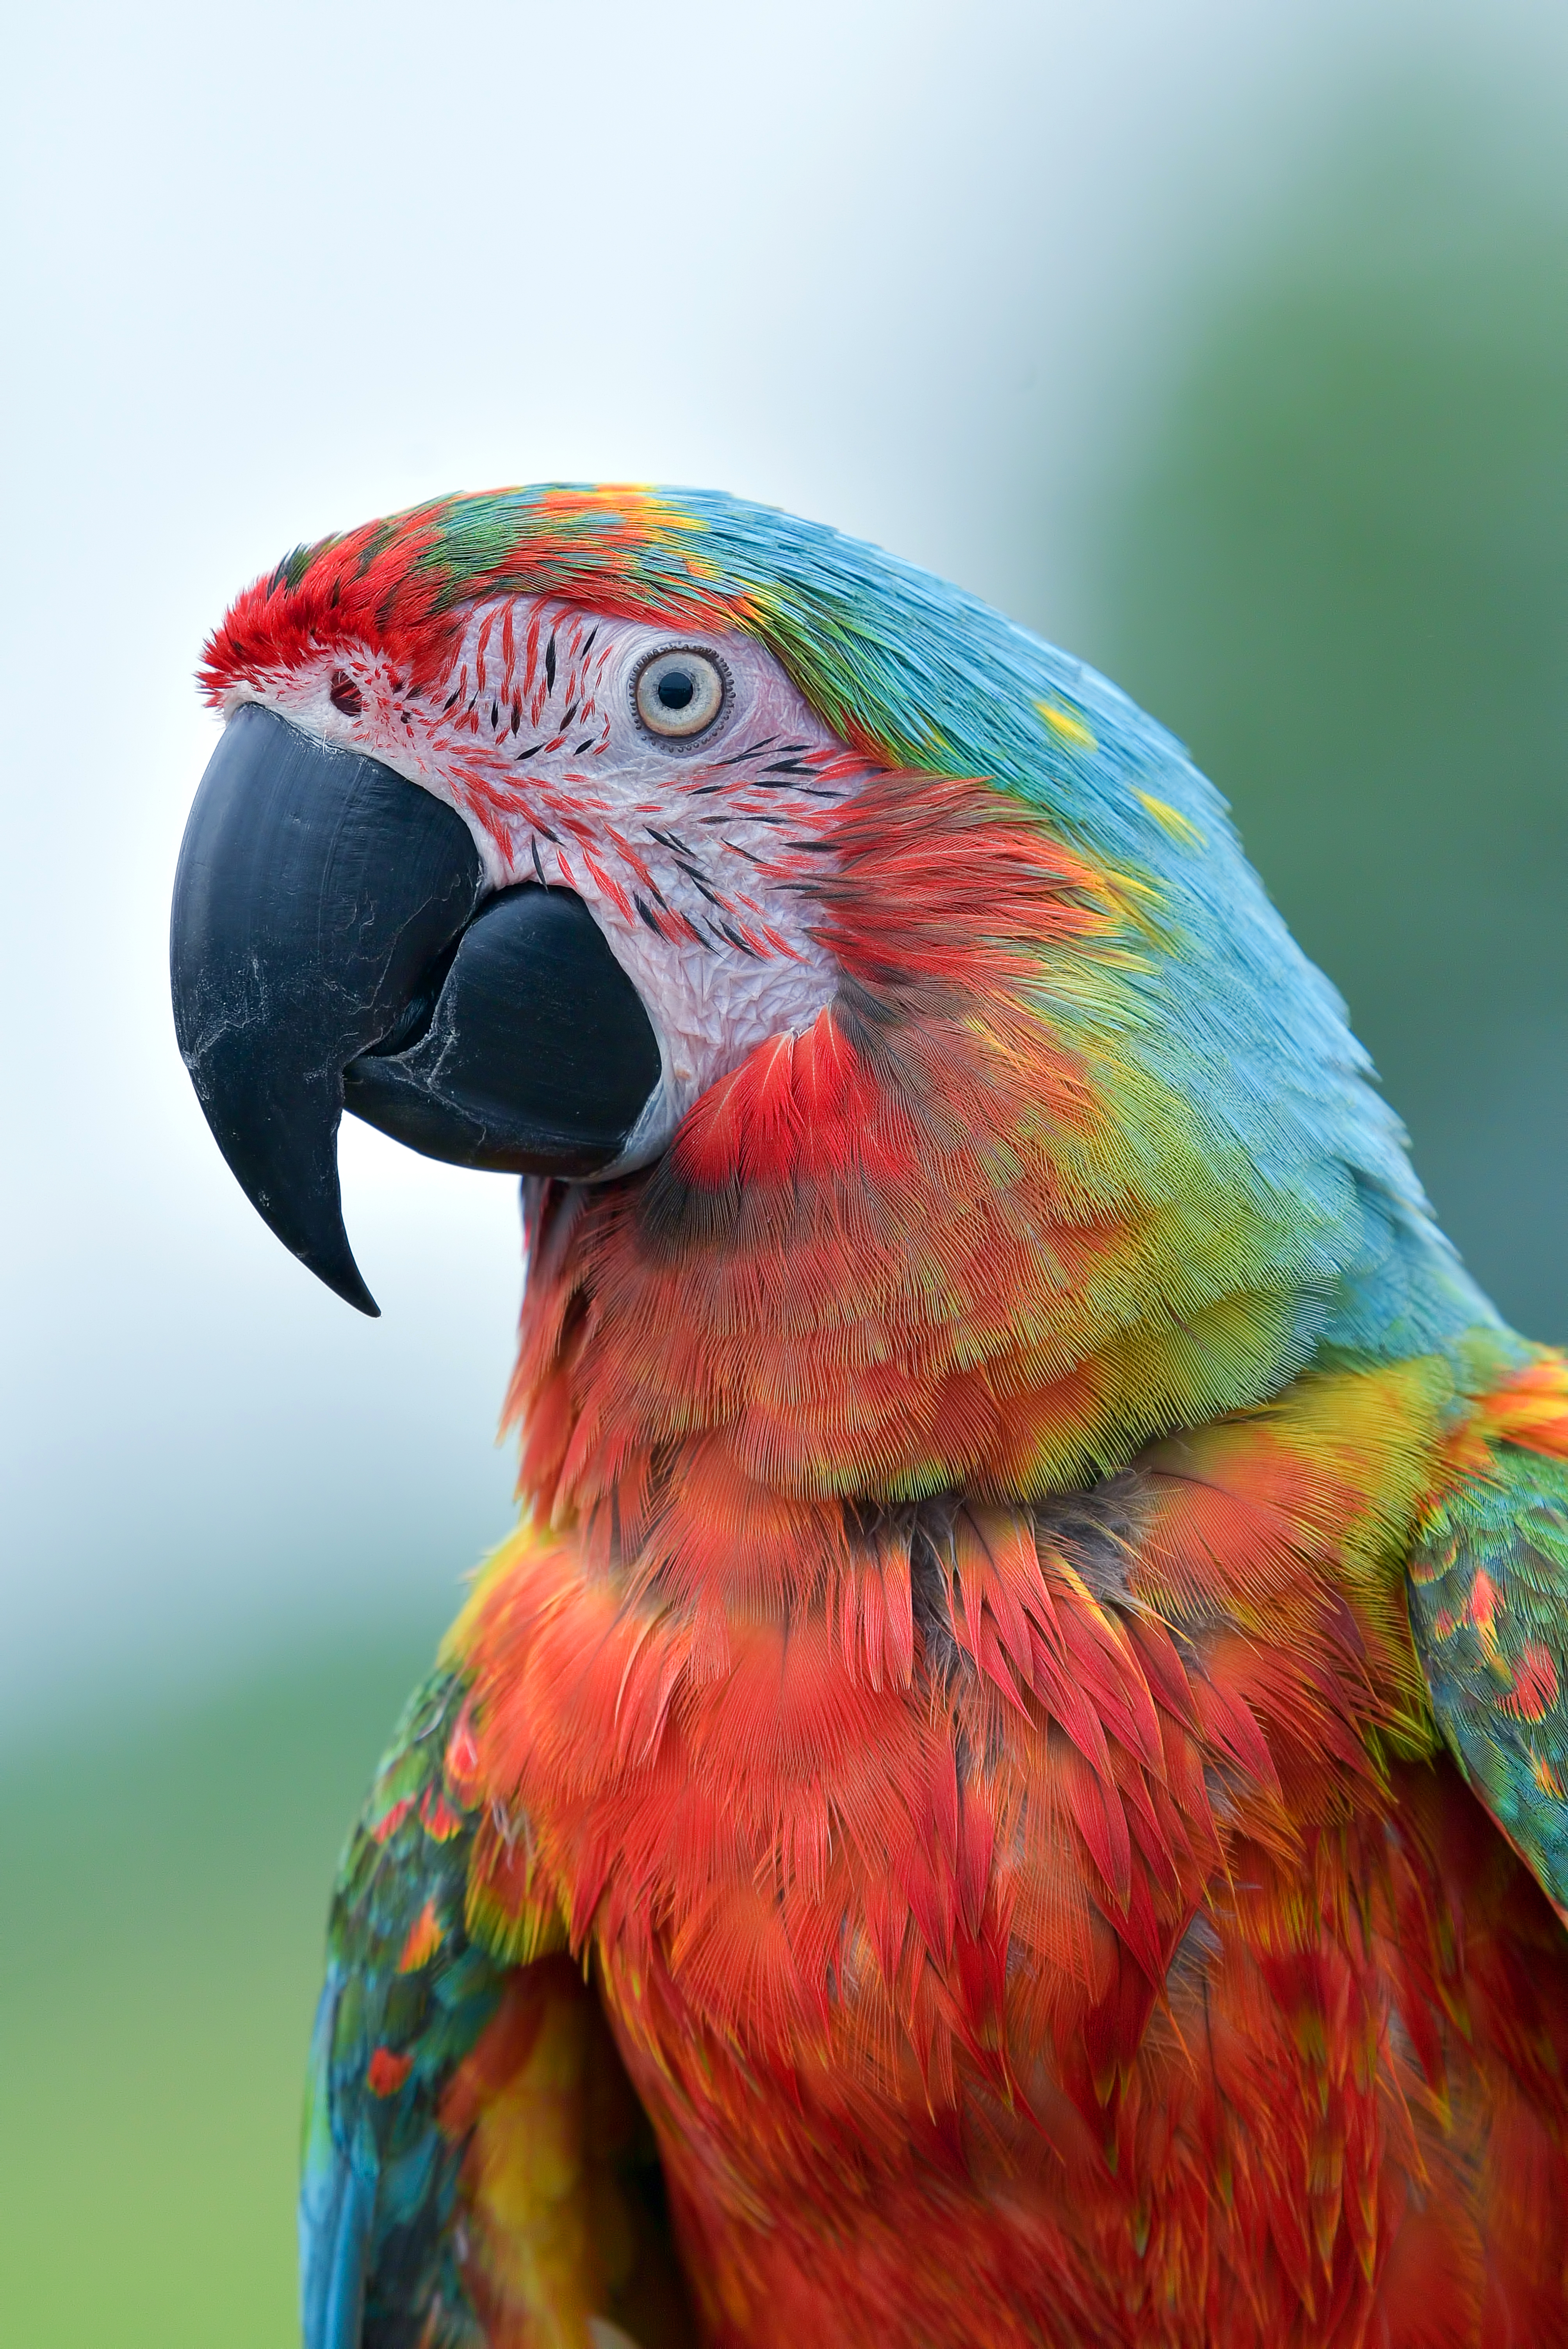
\includegraphics[width=0.2\linewidth]{f.jpg}
    \caption{Maurice Fréchet}
    \label{frechet}
\end{figure}

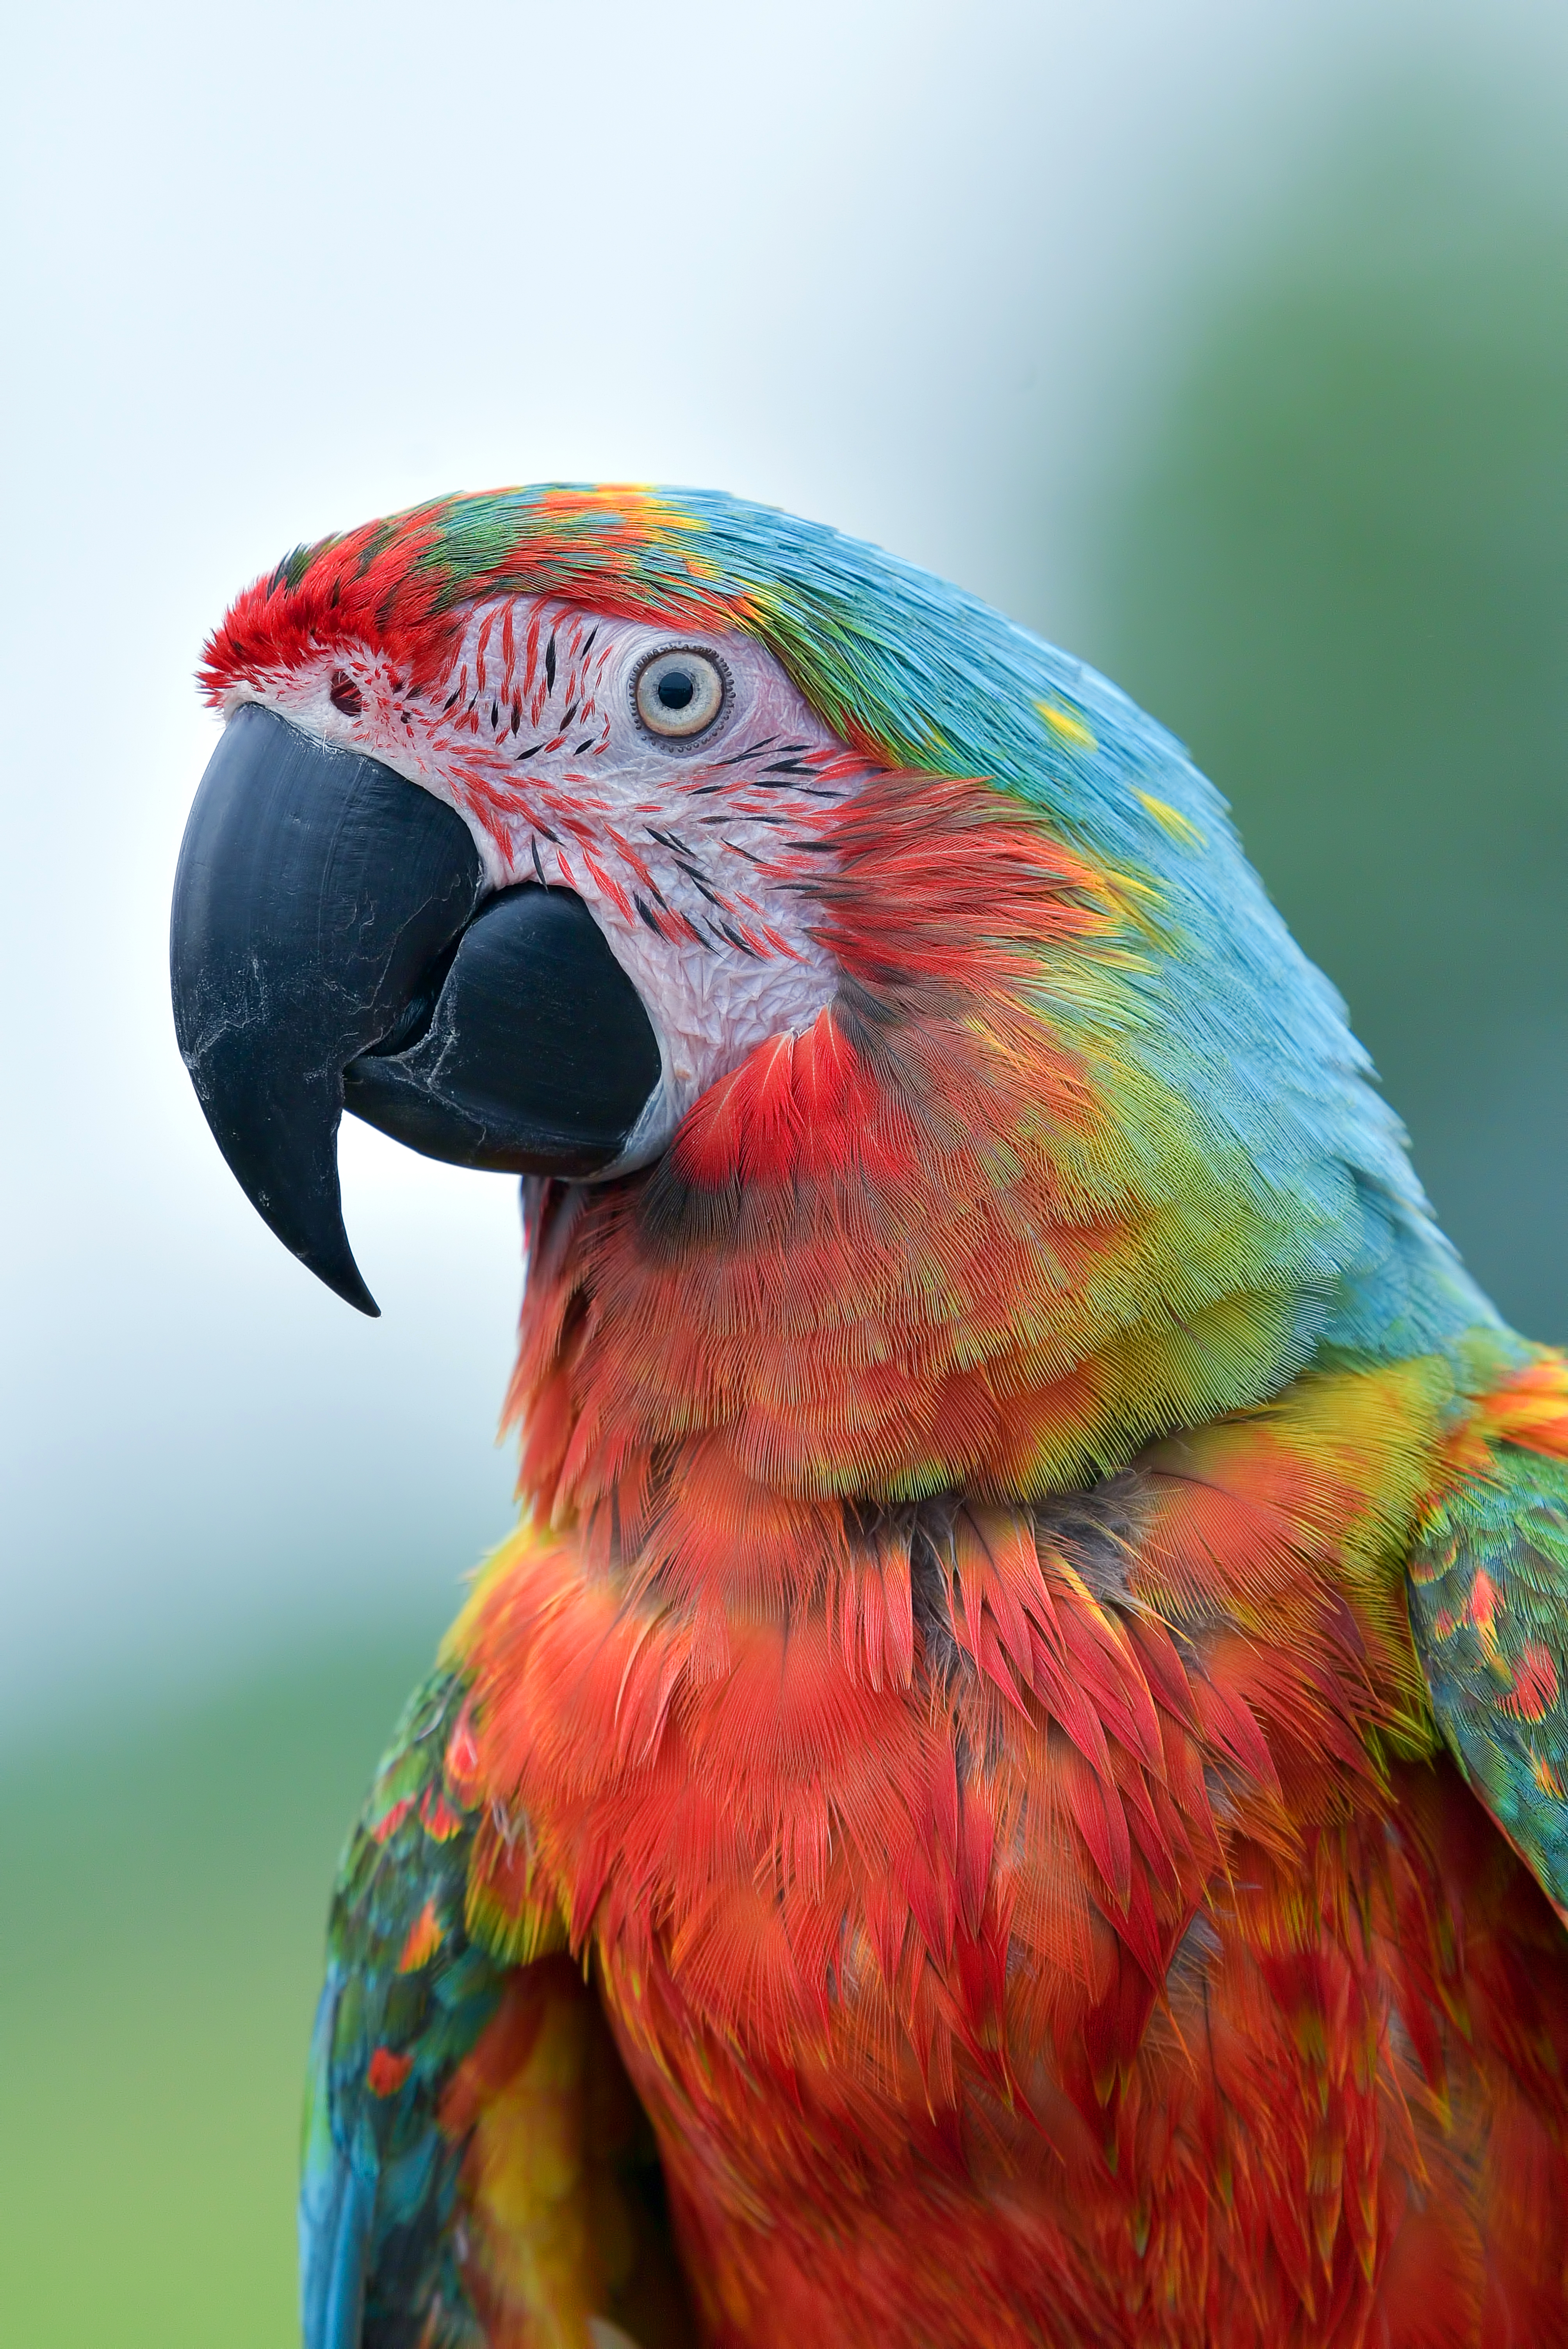
\includegraphics[width=0.8\textwidth]{f.jpg}


\subsection{Varios tipos de gráficos}
Permite diseñar diversos tipos de gráficos con el paquete {\bfseries{\sffamily tikZ}}


\begin{tikzpicture}[domain=0:4]
    \draw[->] (-0.2,0) -- (4.2,0) node[right] {$x$};
    \draw[->] (0,-1.2) -- (0,4.2) node[above] {$f(x)$};
    \draw[color=red] plot (\x,\x) node[right] {$f(x) =x$};
% \x r means to convert '\x' from degrees to _r_adians:
    \draw[color=blue] plot (\x,{sin(\x r)}) node[right] {$f(x) = \sin x$};
\end{tikzpicture}

\subsection{Diagramas conmutativos}
Se insertan diagramas conmutativos con el paquete {\bfseries {\sffamily tikzcd}}.

\begin{tikzcd}
    A \arrow[rd, red] \arrow[r] & B \arrow[d] \\
& C
\end{tikzcd}
%Aqui no supe como agregar las etiquetas en las flechas



\subsection{Uso de mathtools}
Es una paquetría que nos permite un mejor diseño a la hora de usar ecuaciones:

{\bfseries\itshape Ejemplo 1:}


Sin la función \verb+\mathclap+ del paquete \verb+\mathtools+, se generan espacios adicionales a ambos lados del símbolo de sumatoria debido a los índices situados debajo. Un sencillo comando de mathtools permite condensar el resultado.

\[
P_{e_i,\Delta} = \sum_{\substack{j=1 \\ j\neq k,i}} E_i E_j B_{ij} \cos(\delta_{ij}) \delta_{ij,\Delta} + V_k E_i B_{ik} \cos(\delta_{ik,0}) \delta_{ik,\Delta}
\]
\[
P_{e_i,\Delta} = \sum_{\mathclap{j=1, j\neq k, i}} E_i E_j B_{ij} \cos(\delta_{ij}) \delta_{ij,\Delta} + V_k E_i B_{ik} \cos(\delta_{ik,0}) \delta_{ik,\Delta}
\]


{\bfseries\itshape Ejemplo 2:}

Permite superíndices y subíndices a la izquierda (o después) de un símbolo:
\[
\prescript{238}{92}{\mathbf{O}}
\]


{\bfseries\itshape Ejemplo 3:}

Dibuja una caja alredeor de la ecuación:

\begin{teo}
    Este es mi primer teorema.
\end{teo}
\begin{proof}
    \begin{align*}
\Aboxed{ f(x) & = \int h(x)\, dx} \\
              & = g(x)
\end{align*}
\end{proof}




\nocite{*}


\printbibliography

\end{document}
